\documentclass [a4paper] {article}
\usepackage[utf8]{inputenc}
\title{Ciencia de datos, práctica 6}
\author{Juan Casado Ballesteros, Samuel García Gonzalez, Iván Anaya Martín}
\usepackage{Sweave}
\begin{document}
\maketitle

\begin{abstract}
Nuestra tarea es realizar mejoras de visualización sobre gráficas de libre elección. nos vamos a centrar en gráficas con recta de regresión, puesto 
que consideramos que es una gráfica muy utilizada y su análisis para una mejor visualización de la misma puede resultar muy interesante. 
Hemos realizado diferentes análisis y extraido conclusiones de aspectos muy variados, desde el cambio de los ejes de representación de la gráfica o 
simplificar la información representada hasta analizar las gráficas interactivas.

\end{abstract}

\newpage
\tableofcontents


\newpage
\section{Visualización de la regresión}


\section{Mejora de visualización en gráficas con recta de regresión}
La recta de ajuste entre variables es una herramienta muy importante en el análisis de datos y su visualización, pero no lo más importante, puesto que 
si la correlación es baja esta puede no significar nada, asi que lo realmente relevante son la relación entre la recta y los datos. 
Estas nos ofrecen la oportunidad de condensar la información representada de manera muy simple y rápida de ver, facilitando así 
el entendimiento de los datos que se están mostrando. También es interesante porque podemos extraer conclusiones que 
a primera vista no hemos sido capaces de observar. 
Deben poder visualizarse ambos elementos de forma adecuada pues es la relación entre ambos la que nos interesa, deseamos ver lo bien o mal que la recta se adapte a nuestros datos.

En el análisis de regresión compareremos como dos variables de la siguiente muestra se relacionan entre ellas.
Estos datos representan la relación existente entre la población de un país y el tamaño de su parlamento. Hemos escogido datos de 29 países en los
que su sistema político se basa en la democracia liberal.

\begin{Schunk}
\begin{Sinput}
> data <- read.table('democracia.txt')
> data
\end{Sinput}
\begin{Soutput}
   Asientos Poblacion
1       169   5033665
2        63    320040
3       349   9522814
4       120   4027920
5       179   5543451
6       308  33476520
7       158   4367120
8       200   5180000
9       151  24600014
10      200   8000000
11      150  16729950
12       60    509040
13      709  91106500
14       99   3286305
15      183   8032785
16       65   1144910
17       69    410550
18      350  46162900
19       57   4301676
20      650  62261550
21      300  50007300
22      475 126721925
23      101   1294214
24      155  22478255
25      435 314346660
26       72    359280
27      230  10561600
28       63   2029293
29      348  65349876
\end{Soutput}
\end{Schunk}

Para asegurar la calidad en representaciones de regresiones lineales: Estos diagramas se usan para relaciones entre dos variables, 
y nos permiten extraer mucha más información que sólo ver los datos, y de una manera muy accesible y rápida y facilitando la extracción de 
conclusiones. Hay que tener en cuenta que una buena representación de datos debe ser limpia y que a la vez facilite la comprensión de la 
mayor cantidad de información en el menor tiempo posible. Este objetivo lo queremos cumplir en todas las representaciones de este apartado.
Pasamos a representar los datos antes mostrados:

\begin{center}
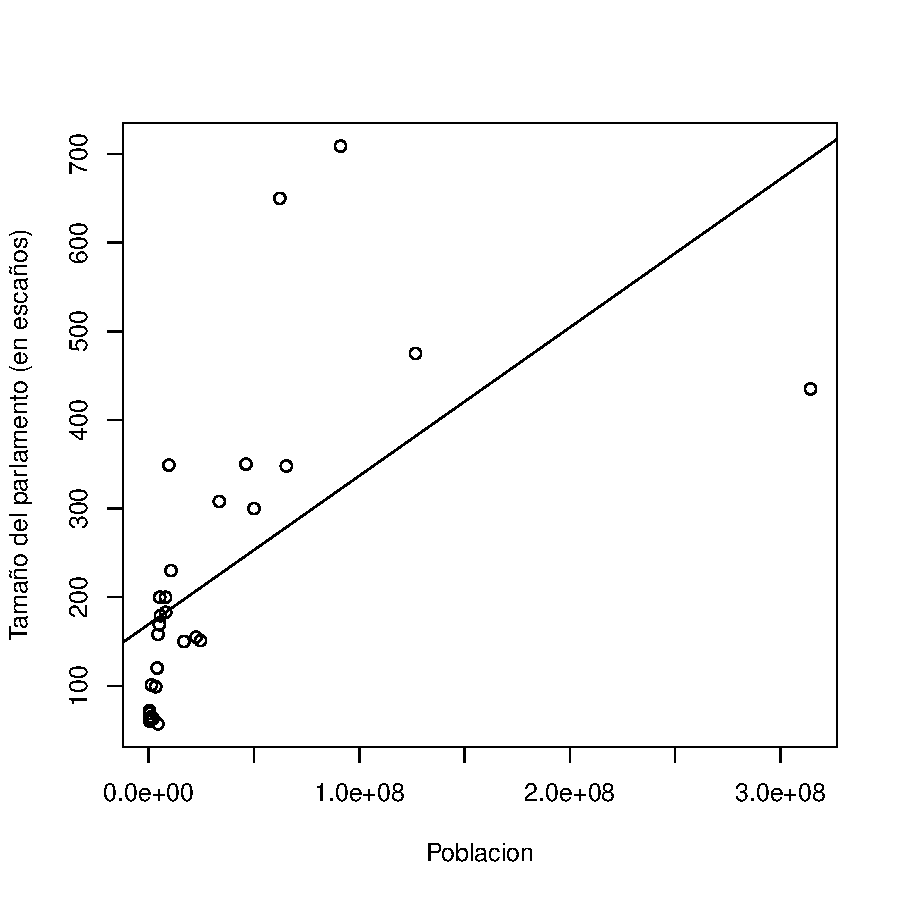
\includegraphics{entrega-plot_democracia}
\end{center}

Es muy importante indicar las unidades de medida en las que representamos los datos, porque modificando estas (sin manipular los datos) 
podemos conseguir una mejor o peor representación de los mismos. Una manera de mejorar esta gráfica es representando las variables de manera 
logarítmica. La usamos con los siguientes propósitos, interpretados de las conclusiones de Edward Tufte en su libro Data Analysis for Politics and Policy: 
\begin{itemize}
  \item Los coeficientes de regresión a veces son más útiles en una interpretación teórica.
  \item Cuando una gráfica está mal distribuida a primera vista y sus datos están agrupados en diferentes clusters, junto con algún dato periférico, se pueden transformar usando en la representación el logaritmo de las observaciones consiguiendo de esta manera que los valores de los clusters se “extiendan” en la gráfica y los valores periféricos se “concentren” también, obteniendo una distribución mucho mejor.
  \item Algunos supuestos teóricos que son fundamentales en el modelo de regresión y su significado en los resultados encajan mejor cuando se usa el logaritmo de las unidades de medida.
\end{itemize}
Estos aspectos que enuncia Tufte, nos benefician en la representación de la muestra que tenemos, puesto que según esas conclusiones (las cuales vamos a probar 
que son ciertas), extraemos que la representación logarítmica de las variables da resultado a una distribución mucho más simétrica, 
puesto que los valores muy grandes los “aplana” hacia la media, y los valores pequeños los “estira”. 
Cabe destacar que transformar las variables usando logaritmos reduce la no-linealidad en la relación y reduce en gran medida el desorden 
en las distribuciones, es decir, ayuda a clarificar la relación entre dos variables. Pasamos a probar estos fundamentos teóricos en la realidad, 
representando la población en escala logarítmica: 

\begin{center}
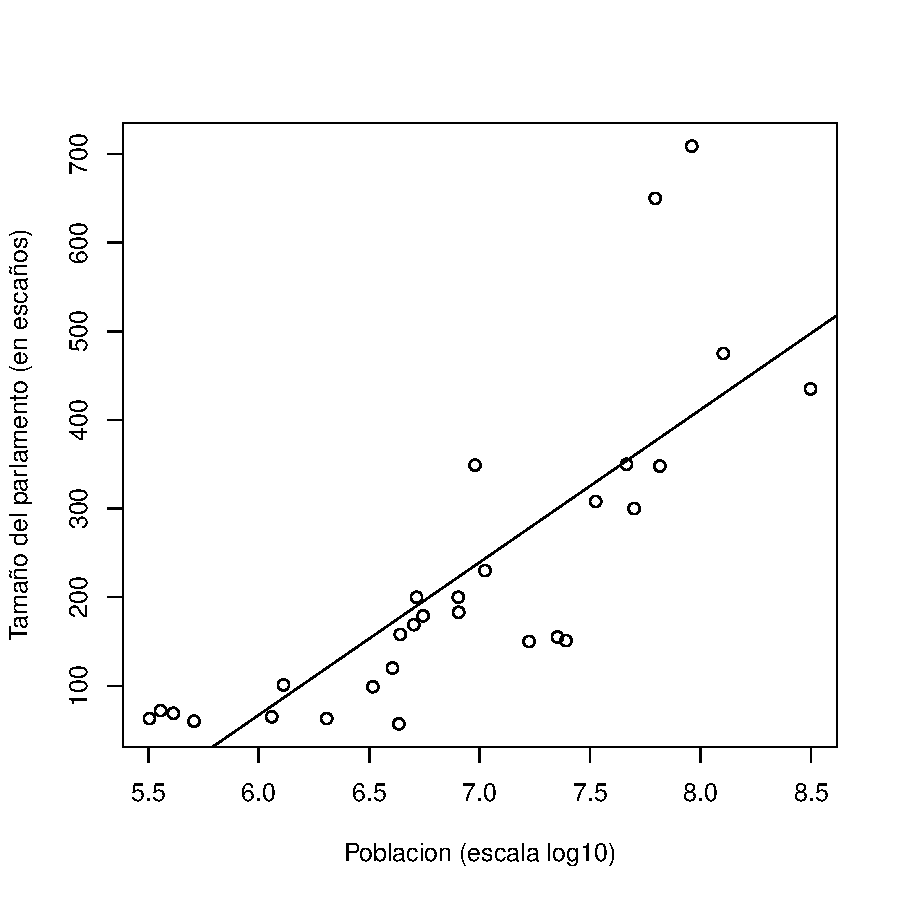
\includegraphics{entrega-plot_democracia_log}
\end{center}

Como podemos ver, es mucho más clara no solo la relación entre las dos variables, pues en la anterior gráfica 
podíamos apreciar que los datos estaban relacionados, sino también la distribución de puntos,  y con mucha diferencia,
puesto que en la anterior gráfica se concentraban mucho en la parte inferior. En la nueva podemos ver que están mucho más repartidos y la comprensión 
a primera vista es más clara y rápida. Este análisis nos demuestra que también se puede mejorar la visualización de 
una gráfica usando otros métodos aparte de la mejora simplemente visual, como hemos hecho en este apartado modificando los ejes de representación.

\subsection{La importancia de la visualización}
Como ejemplo ilustrativo de la importancia de la visualización ponemos el ya famoso ejemplo del libro de Edward Tufte, Data Analysis for Politics and Policy, Chapter 3: Two-Variable Linear Regression.
En dicho ejemplo las rectas de regresión obtenidas son idénticas y se adaptan a ojos de la correlación de igual modo a los datos.
Si no fuera por la visualización de ambos elementos en conjunto no podríamos conocer la gran disparidad entre cada una de las muestras.

Si representáremos los datos solos sería difícil imaginar que tuvieran la misma regresión y si visualizáramos las regresiones solo sería difícil imaginar que podrían estar representando a datos tan dispares.
\begin{Schunk}
\begin{Soutput}
[1] "1: Correlacion cuadrada: 0.6665425 a: 3.000091 b: 0.5000909"
\end{Soutput}
\begin{Soutput}
[1] "2: Correlacion cuadrada: 0.666242 a: 3.000909 b: 0.50"
\end{Soutput}
\begin{Soutput}
[1] "3: Correlacion cuadrada: 0.666324 a: 3.002455 b: 0.4997273"
\end{Soutput}
\begin{Soutput}
[1] "4: Correlacion cuadrada: 0.6667073 a: 3.001727 b: 0.4999091"
\end{Soutput}
\end{Schunk}

\begin{center}
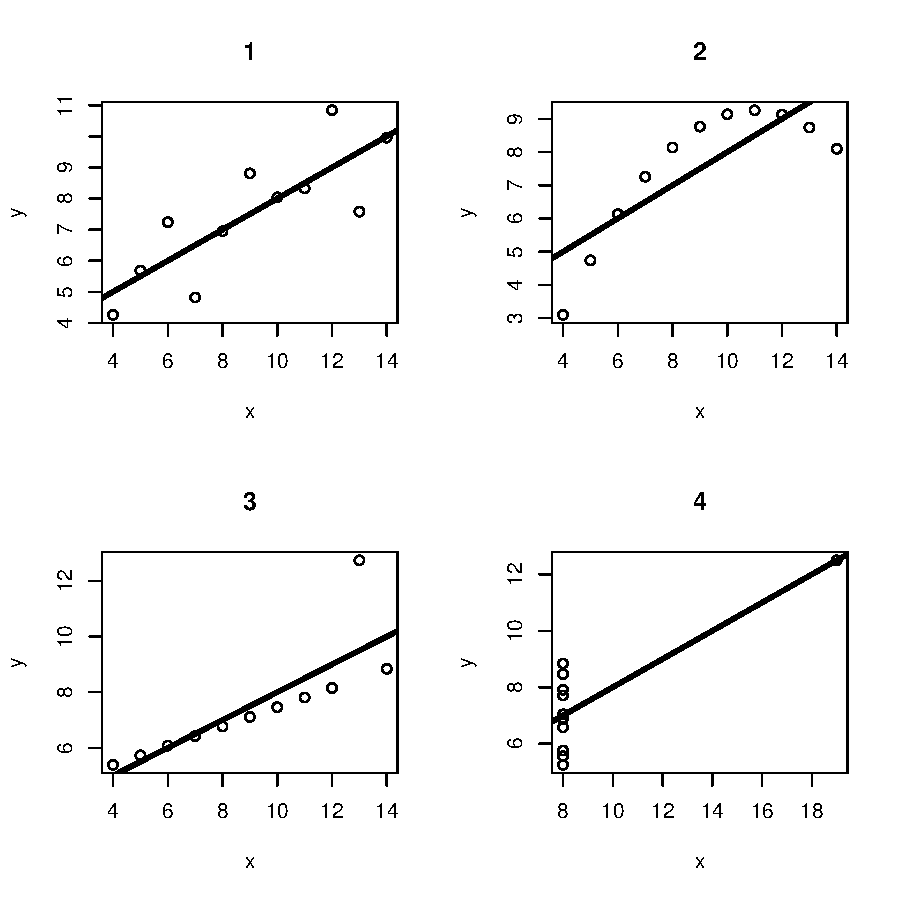
\includegraphics{entrega-plot_regresion4}
\end{center}

\subsection{Cantidad de información mostrada}
Debido a la simpolicidad de esta gráfica, solo se está mostrando una nube de puntos y la recta de regresión es tentador comenzar a añadir elementos adicionales.
No obstante antes de hacerlo debemos tener en cuenta las siguientes consideraciones.
\begin{itemize}
  \item Se debe mostrar la información mínima necesaria para mostrar aquello que deseamos.
        Si tenmos que mostrar una relación compleja entre los datos puede que sea necesario utilizar una representación compleja.
        No obstante si podemos hacerla simple será mejor pues podrá ser entendida por más gente de forma más rápida.
  \item Debemos de indicar el significado de cada elemento que añadamos a la gráfica cuando este no sea claro.
  \item Es de gran importancia indicar la margnitud de los datos tanto como el dato que se está representando en cada eje.
\end{itemize}


\begin{Schunk}
\begin{Soutput}
[1] "Correlacion cuadrada de Temperaturas: 0.835327071582904"
\end{Soutput}
\end{Schunk}

En este caso mostramos exclusivamente los datos jusnto a su recta de regresión.
Obtenemos una representación muy clara y sencilla que nos muestra directamente la información que queríamos.
La gráfica tiene un título y en cada eje mostramos la variable representada y las unidades de esta.
\begin{center}
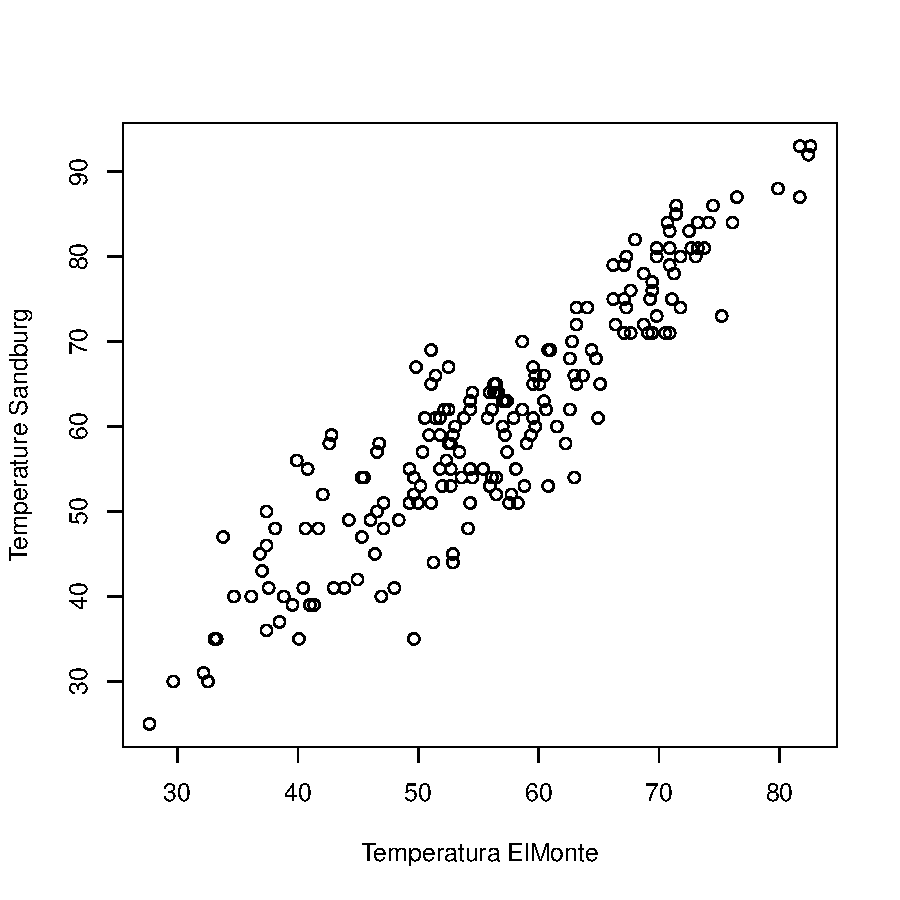
\includegraphics{entrega-temp_plot}
\end{center}
Podemos aumentar la complejidad de la representación añadiendo dos líneas paralelas a la recta de regresión que nos indiquen la desviación típica de esta.
Este elemento adicional nos proporciona información adicional sobre la regresión que dependiendo del contexto puede ser necesaria si a partir de los datos y de la recta es difícil juzgar la calidad de esta.
No obstante podemos ver como solo con haber añadido un elemento tan simple la representación se siente mucho más densa.
\begin{center}
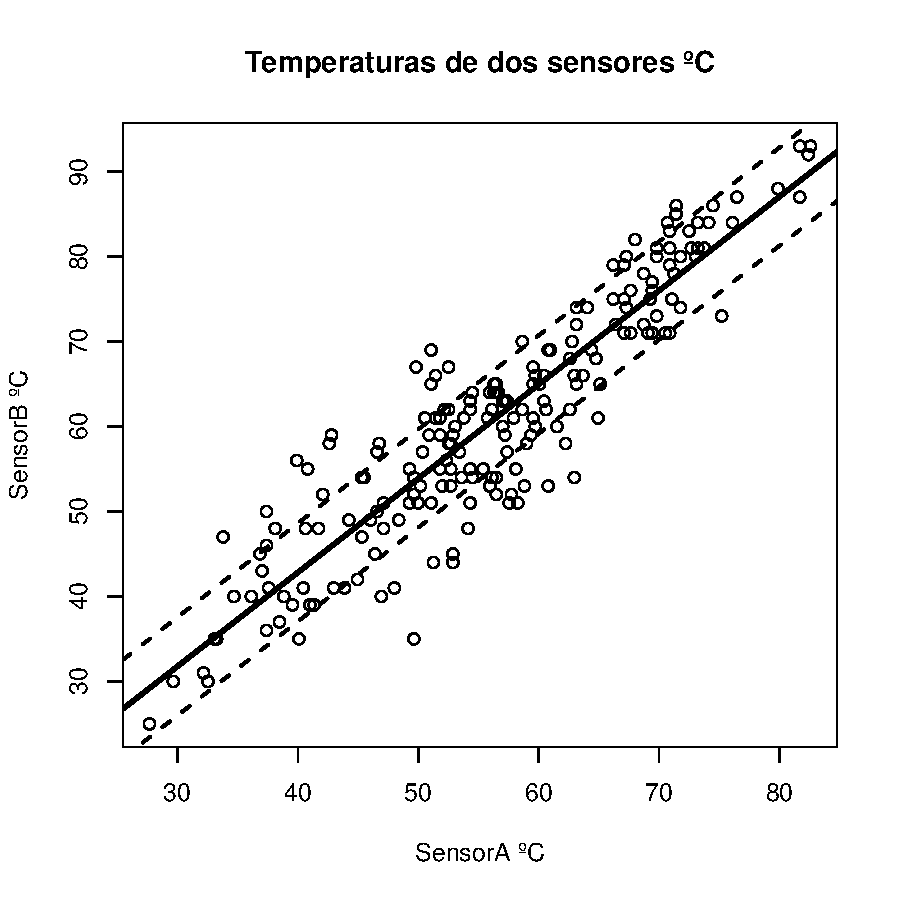
\includegraphics{entrega-temp_reg_plot}
\end{center}

Como hemos indicado para este caso sería recomendable añadir una leyenda que nos indicara qué datos se estan representando de modo que la visualización obtenida sea más clara.
\begin{center}
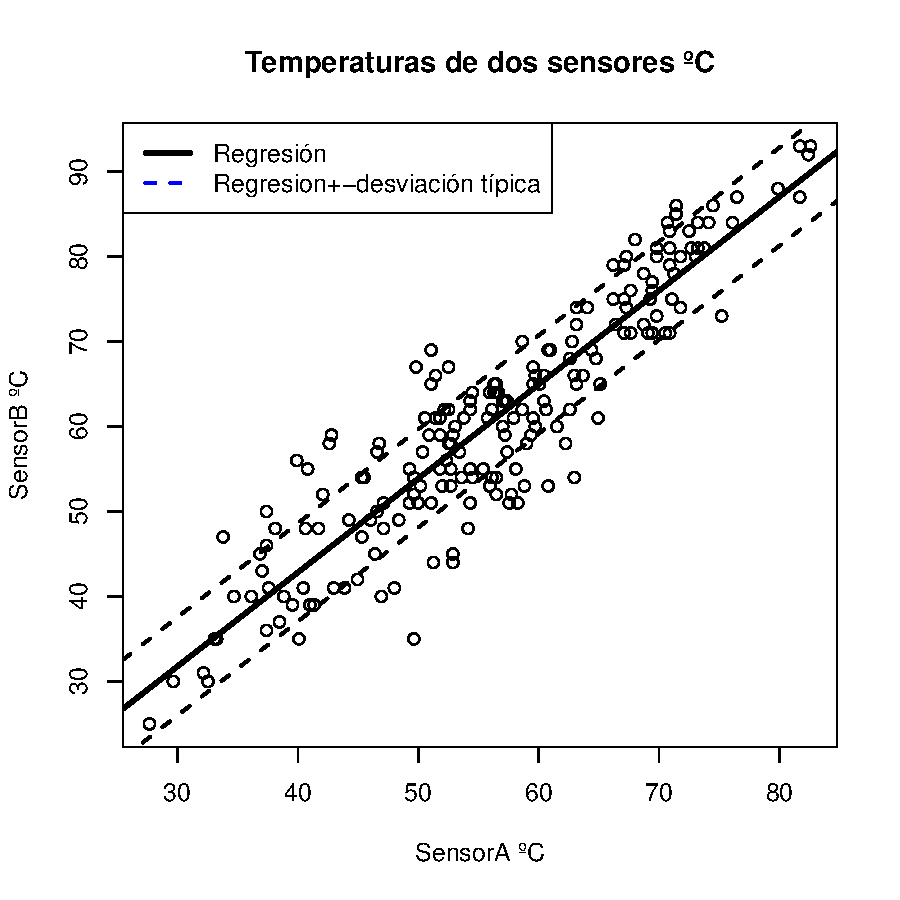
\includegraphics{entrega-temp_plot_legend}
\end{center}

\subsection{Paquetes de visualización}
Para realizar las gráficas anteriores hemos utilizado la siguiente función que utiliza las funciones propias de R.
\begin{Schunk}
\begin{Sinput}
> regPlot
\end{Sinput}
\begin{Soutput}
function (x, y, regresion, limit, title="", xlabel="", ylabel="") {
  plot(x, y, xlab=xlabel, ylab=ylabel, main=title)
  regUpLimit <- regresion
  regUpLimit$coefficients[1] = regUpLimit$coefficients[1] + limit
  regDownLimit <- regresion
  regDownLimit$coefficients[1] = regDownLimit$coefficients[1] - limit
  abline(regUpLimit, "gray", lty=2, lwd=2)
  abline(regresion, "black", lty=1, lwd=3)
  abline(regDownLimit, "gray", lty=2, lwd=2)
}
<bytecode: 0x000001f9c42e5990>
\end{Soutput}
\end{Schunk}
Mediante plot visualizamos la nube de puntos y con abline dibujamos líneas rectas sobre la última gráfica creada.

Existen una gran cantidad de paquetes que se pueden utilizar para visualizar datos.
Uno de los más famosos es "ggPlot2".
Esto se debe a que produce gráficas muy vistosas, altamente configurables todo con una sintaxis sencilla y fácil de aprender.

No obstante esto también es uno de los problemas de esta librería.
Por defecto las gráficas que obtendremos tendrán un fóndo grisáceo con una cuadrícula en blanco tal y como podemos ver en el ejemplo.
Esto hace que la representaciín de los datos sea más difusa que la obtenida con las funciones propias de R que crean una visualización mucho más limpia.
\begin{center}
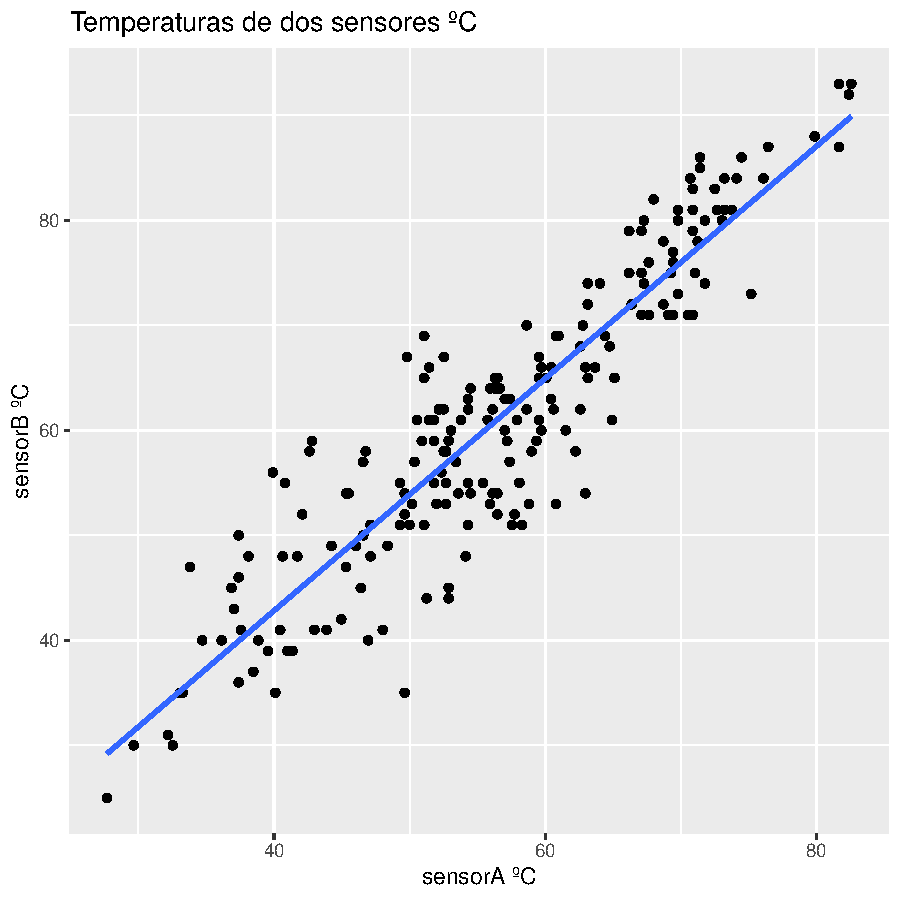
\includegraphics{entrega-ggplot2_NO_se}
\end{center}

Estas librería permite además añadir gran variedad de elementos de forma sencilla a las gráficas.
Dichos elementos se ven siempre muy vistosos y bonitos pero pueden no tener gran significado para nuestro caso concreto.
Debemos por tanto tener cuidado y no abusar de ellos.
\begin{center}
\begin{Schunk}
\begin{Sinput}
> ggplot(data = datos3, aes(x = datos3$Temperature_ElMonte, 
+                           y = datos3$Temperature_Sandburg)) + 
+   geom_point(color='black')+
+   geom_smooth(method="lm")+ 
+   labs(title = "Temperaturas de dos sensores ºC") +
+   xlab("sensorA ºC") + ylab("sensorB ºC")
\end{Sinput}
\end{Schunk}
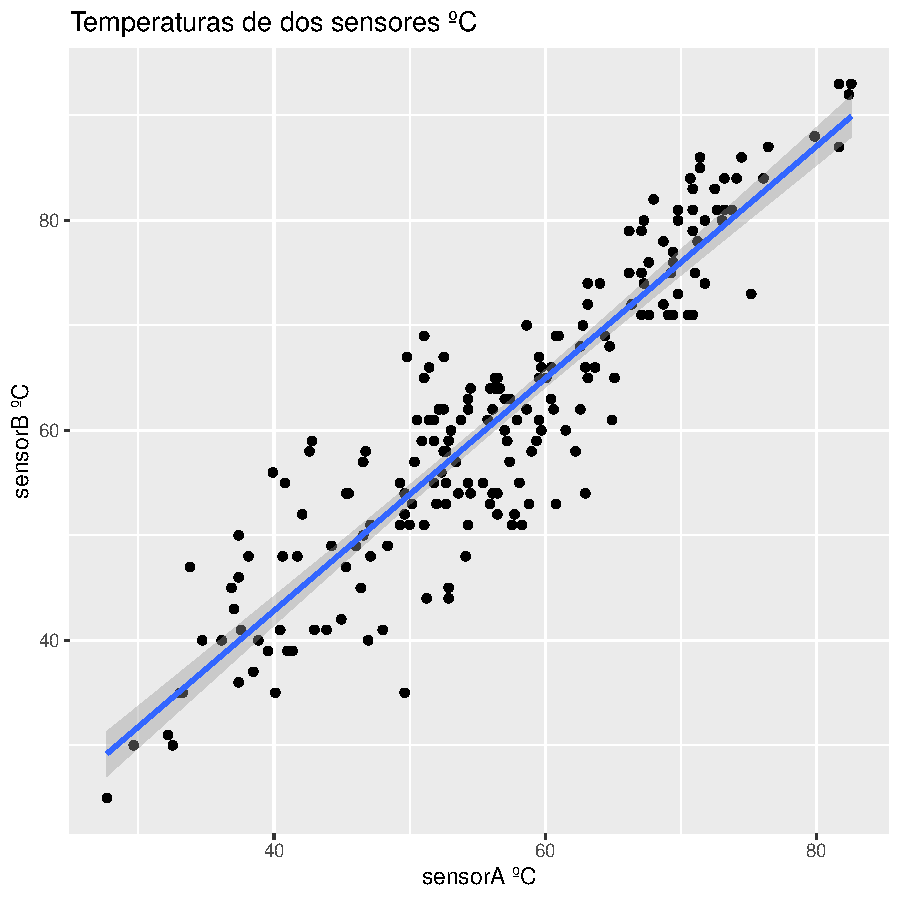
\includegraphics{entrega-ggplot2_se}
\end{center}

\subsubsection{Representaciones interactivas}
Una de las ventajas que tenmos con estas librerías es que podemos crear gráficas interactivas.
Estas gráficas crean un archivo .html que podemos visualizar de forma interactiva en el navegador.
Las gráficas interactivas nos permiten realizar representaciones más complejas de los datos así como representar más datos a la vez.
Esto se debe a que cualdo pasemos el cursosr encima de los elementos se resaltarán los que están relacionados pudiendo ver simultáneamente estos con respecto a los otros.

Mostramos uan gráfica creada con "ggplot2" que se ha convertido en una gráfica interactiva con "ggiraphExtra".
\begin{center}
  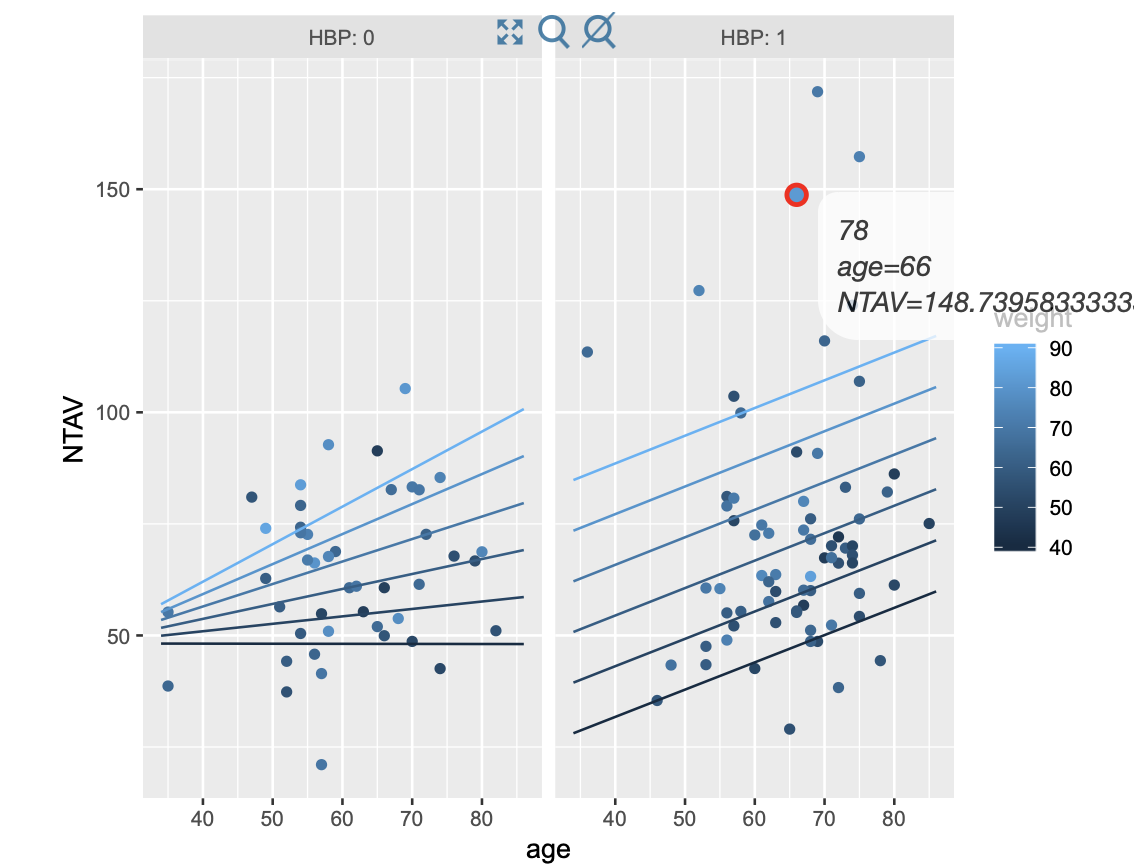
\includegraphics{interactive.png}
\end{center}

En este caso mostramos una gráfica interactiva creada con "plotly" la cual utiliza "ggplot2" por debajo para crear sus gráficas.
Esta librería tiene también una sintaxis sencilla y permite crear grácisas muy configurables.
Como ventaja frente a "ggplot2" debemos comentar que los estilos que se aplican por defecto a las gráficas son mucho más limpios y claros.
\begin{Schunk}
\begin{Sinput}
> datos3 %>%
+   plot_ly(x = ~Temperature_ElMonte, y = ~Temperature_Sandburg) %>%
+   add_markers (x = ~Temperature_ElMonte, y = ~Temperature_Sandburg, 
+     name="temperaturas ºC") %>%
+   add_lines(x = ~Temperature_ElMonte, y = fitted(regresion3), name="regresion")%>%
+   layout(title = "Temperaturas de dos sensores ºC",
+     xaxis = list(title = "sensorA ºC"),
+     yaxis = list(title = "sensorB ºC"))
\end{Sinput}
\end{Schunk}

\begin{center}
  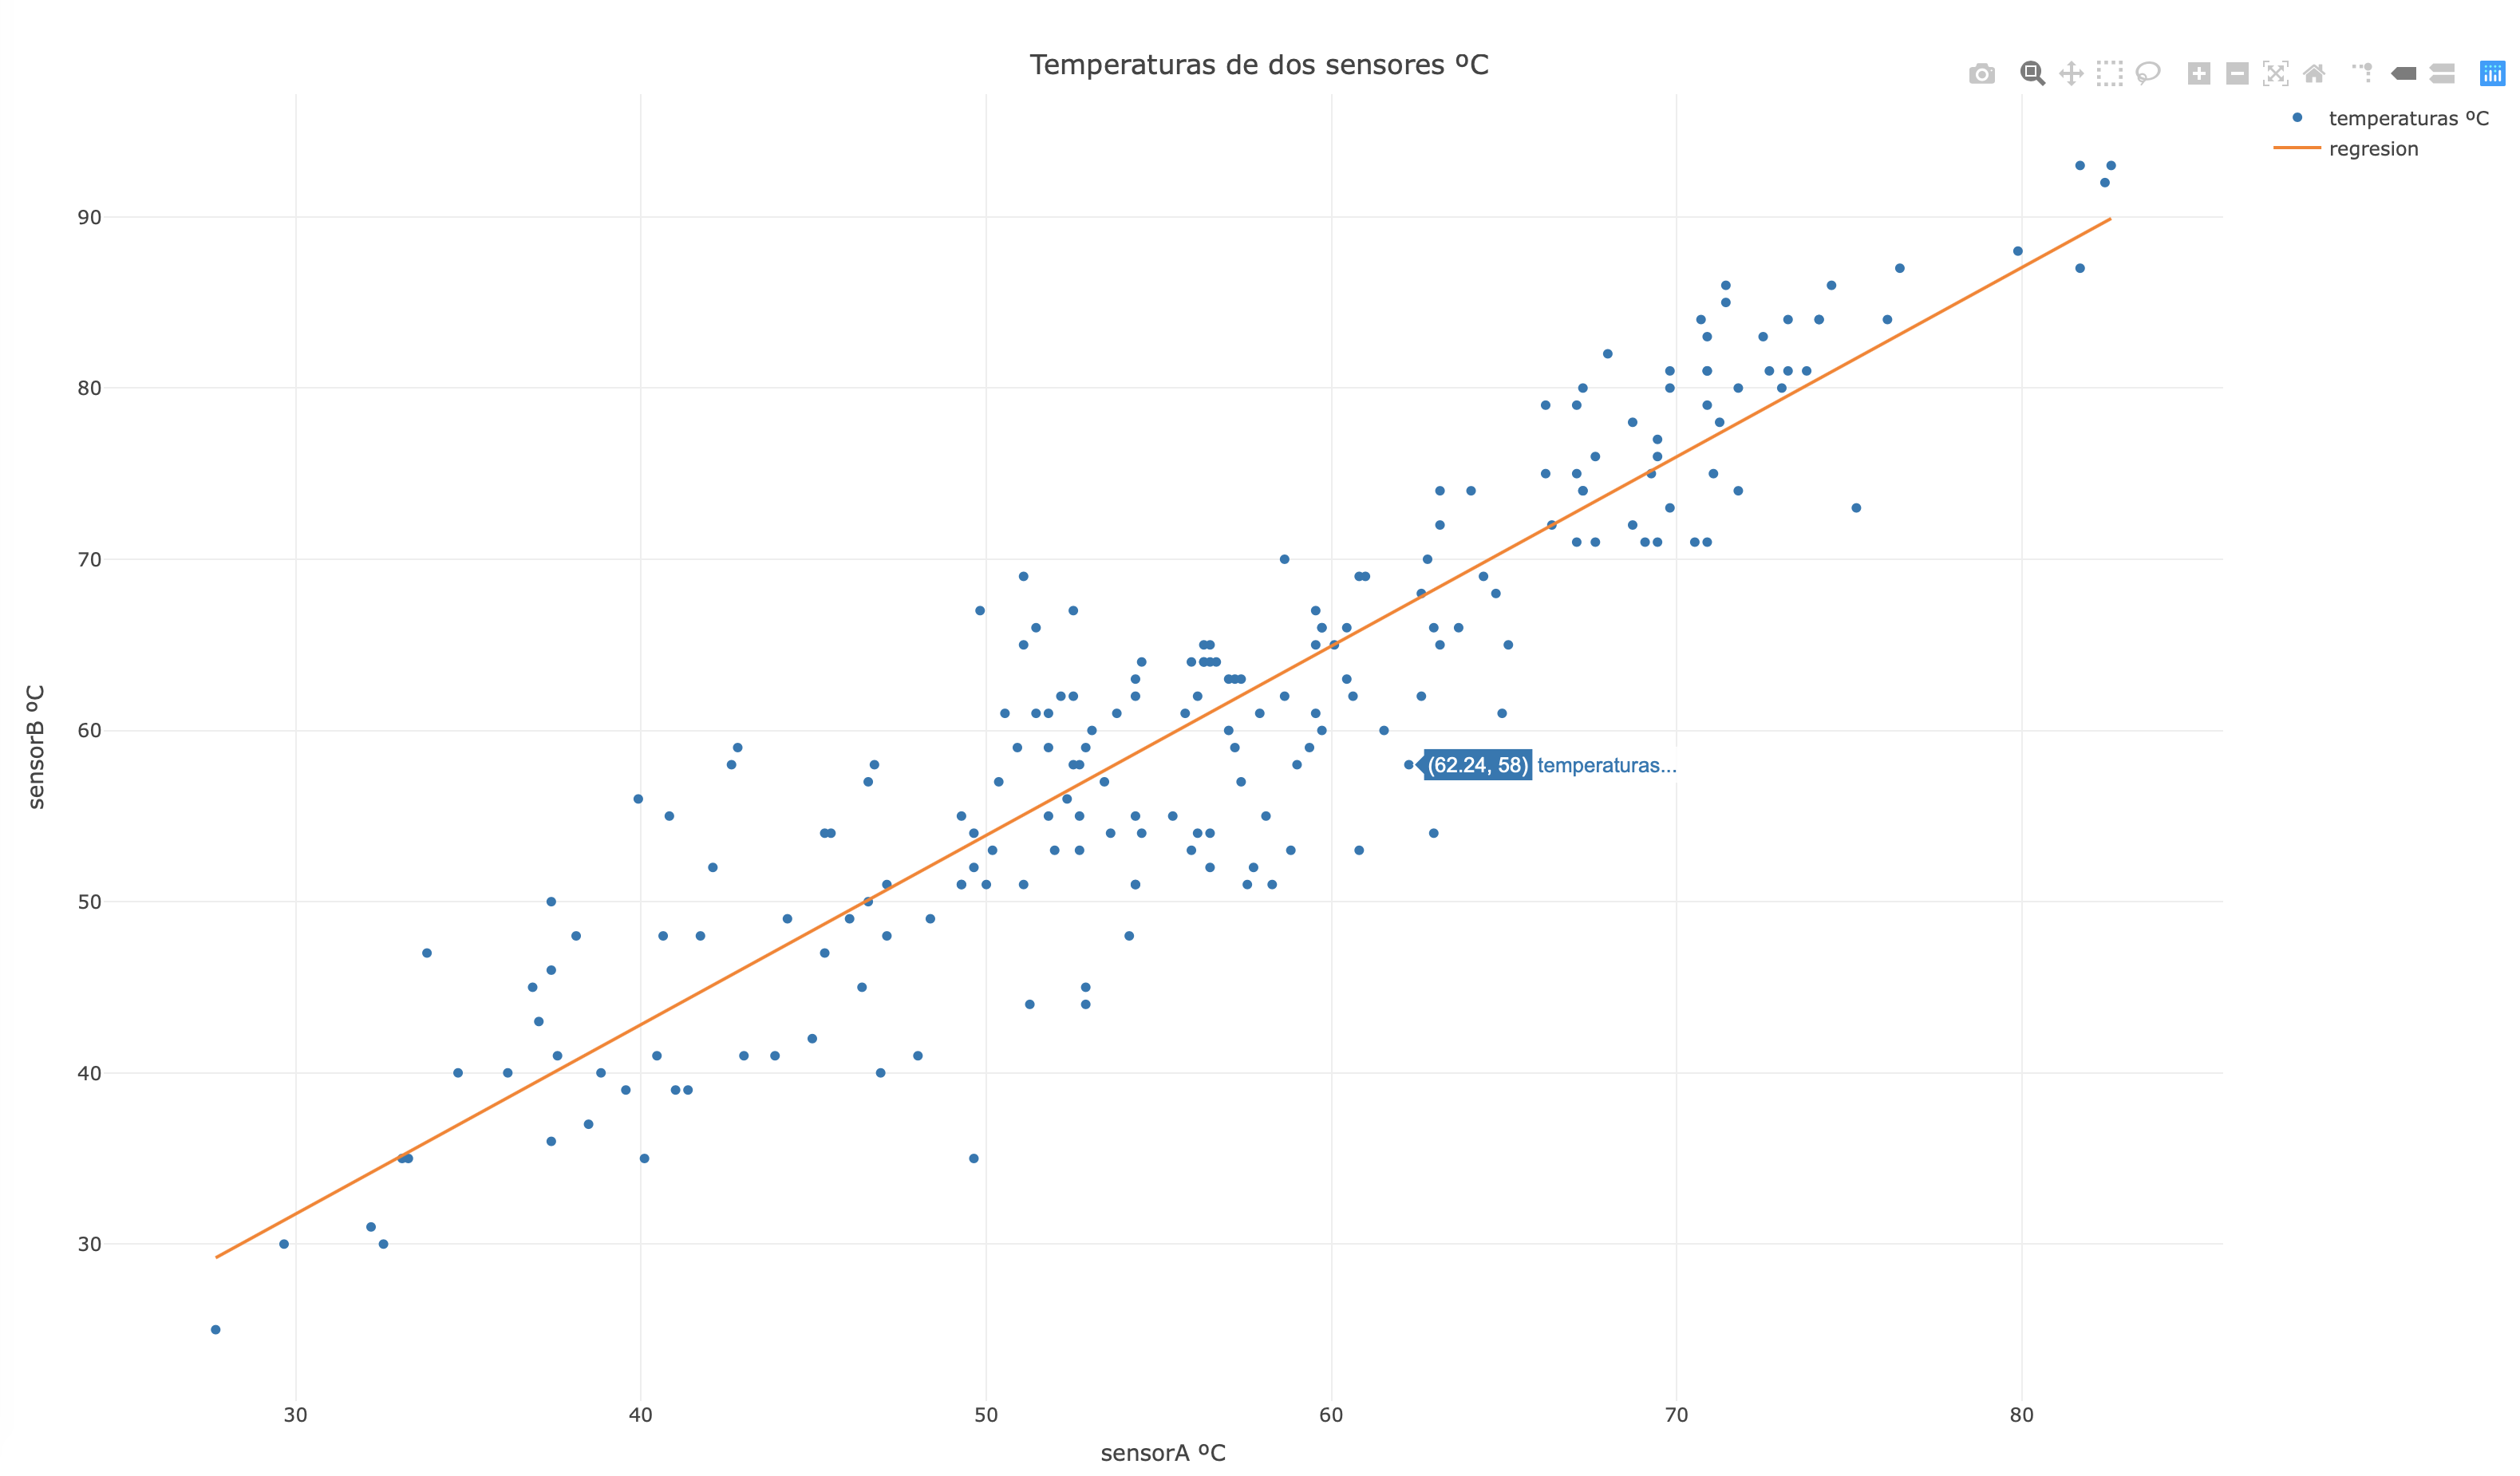
\includegraphics{interactive2.png}
\end{center}

\end{document}
